\begin{figure}[t]
  \centering
  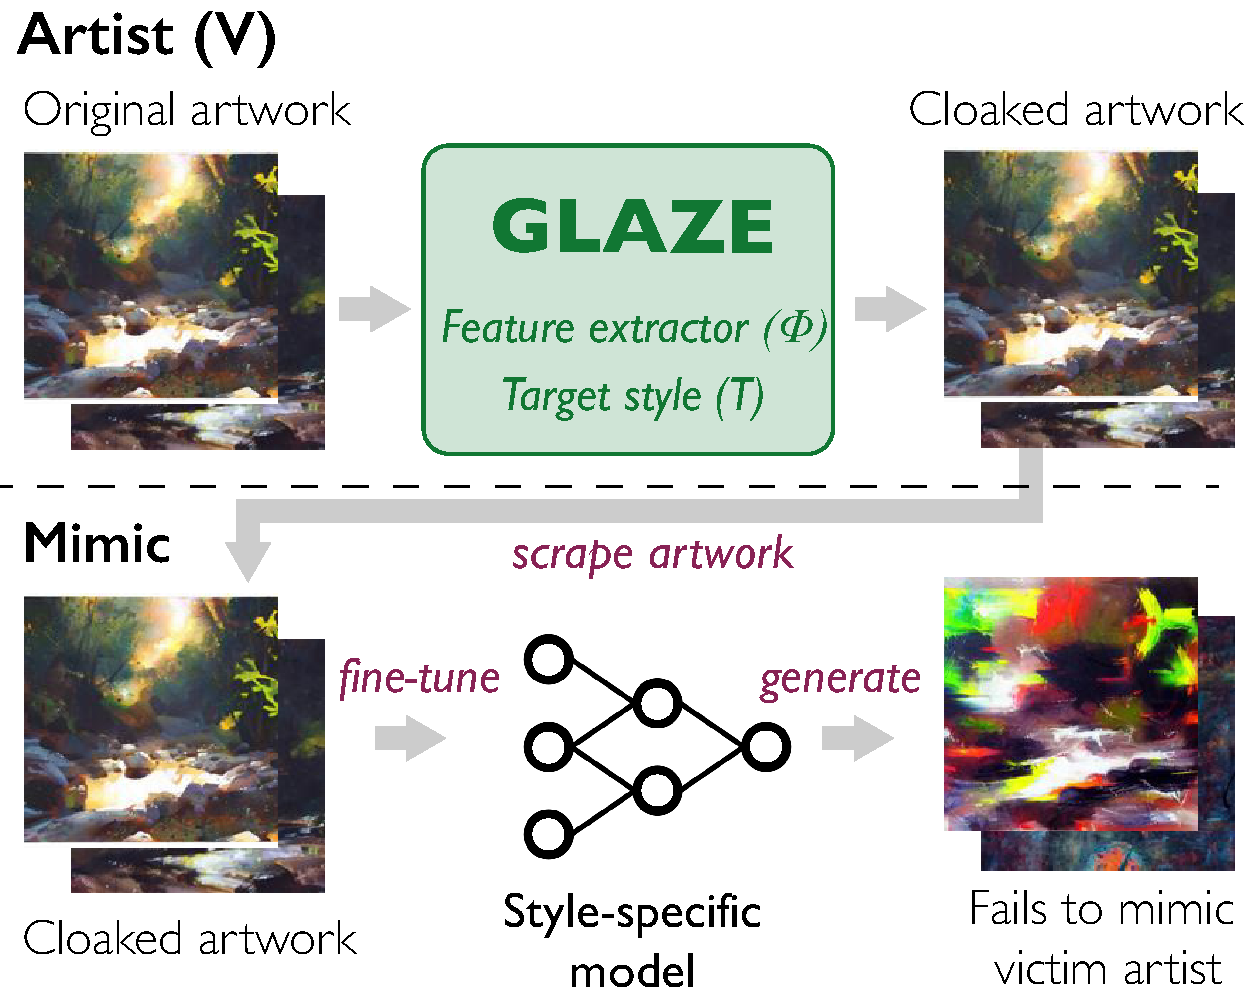
\includegraphics[width=0.9\columnwidth]{plots/overview/cloak-scenario-emily.pdf}
  \caption{Overview of \system{}, a system that protects victim artists from AI style mimicry by cloaking their online artwork. ({\bf Top}) An artist $V$ applies the cloaking algorithm (uses a feature extractor $\Phi$ and a target style $T$) to generate cloaked versions of $V$'s art pieces. Each cloak is a small perturbation unnoticeable to human eye. ({\bf Bottom}) A mimic scrapes the cloaked art pieces from online and uses them to fine-tune a model to mimic $V$'s style. When prompted to generate artwork in the style of $V$, mimic's model will generate artwork in the target style $T$, rather than $V$'s true style. }
  \label{fig:cloaking}
\end{figure}

\begin{figure}[t]
  \centering
  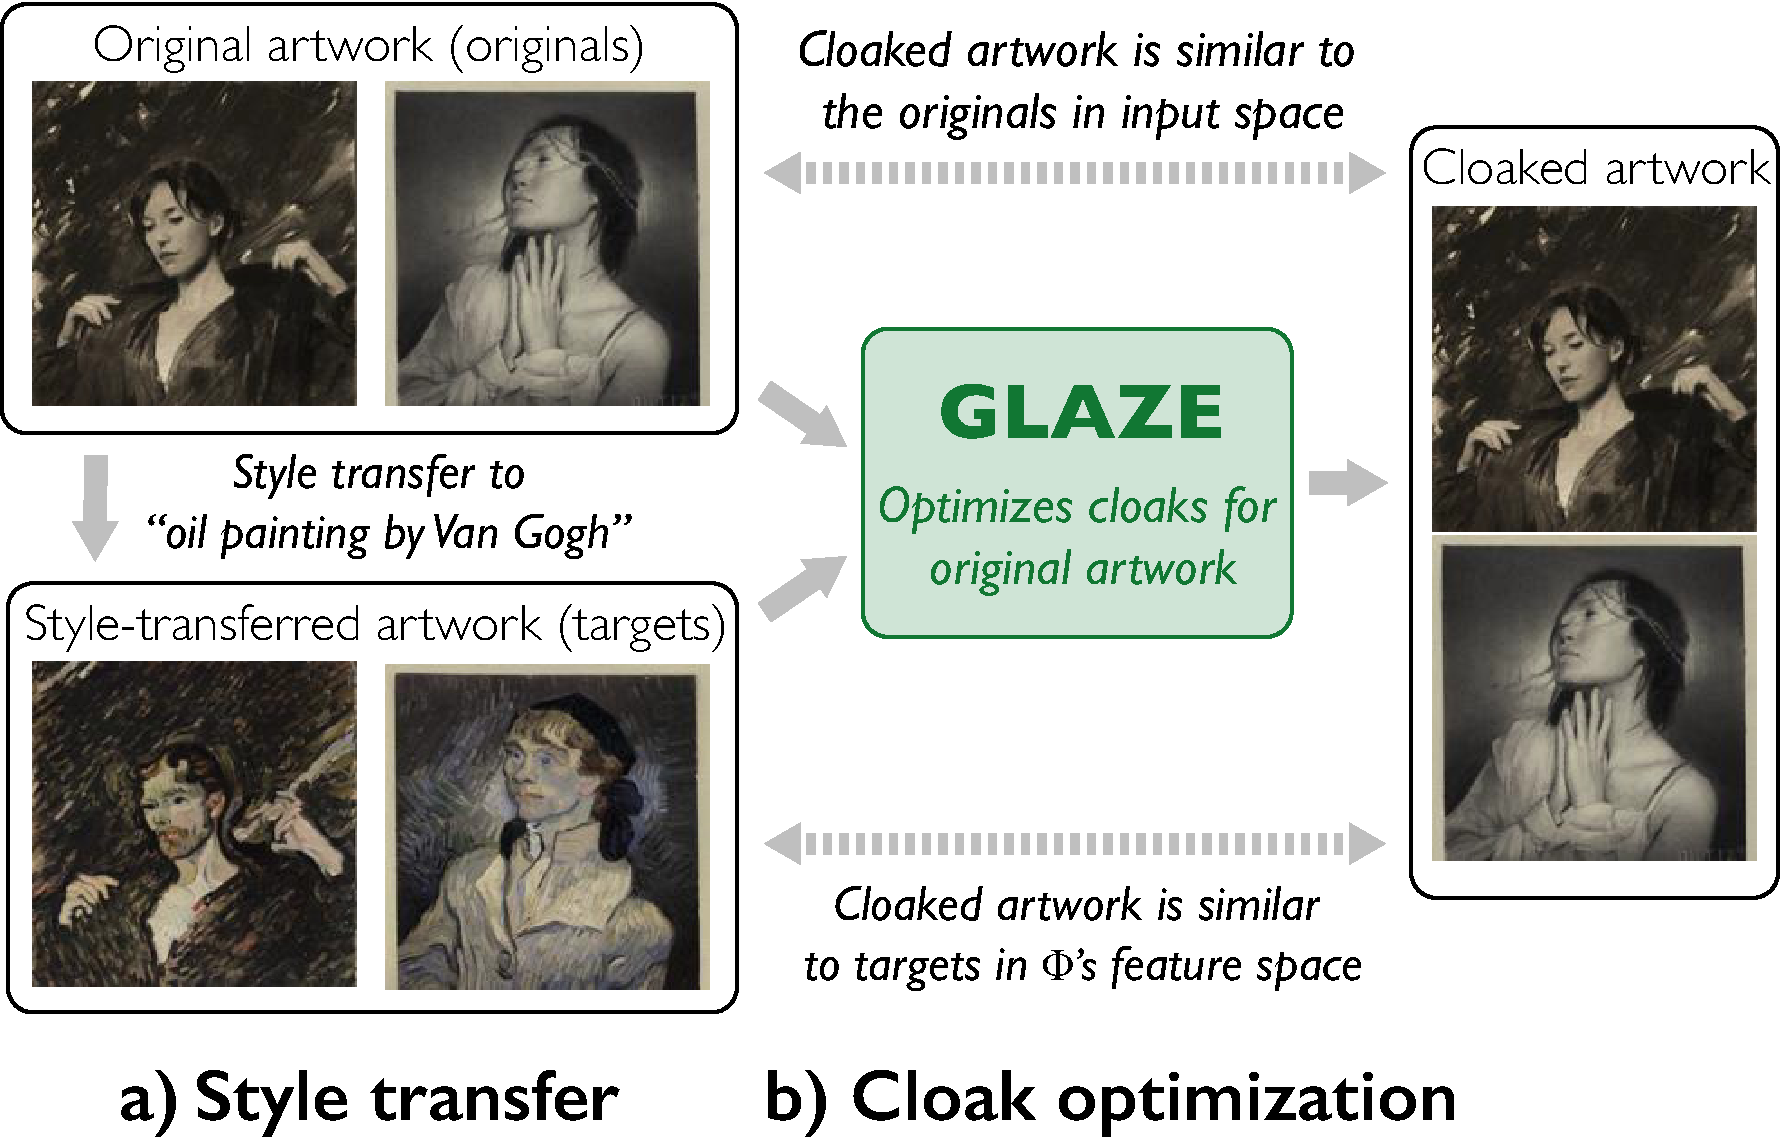
\includegraphics[width=1\columnwidth]{plots/overview/cloak-intuition-2-emily.pdf}
  \caption{High level overview of how \system{} perturbs the style-specific features of the artwork. {\bf a)} \system{} style transfers the original artwork to a different style, which changes its style but leaves other features unaltered. {\bf b)} \system{} optimizes a cloak that makes the artwork's features representation match that of the style-transferred art, while constraining the amount of visible changes to the artwork.  }
  \label{fig:cloak-intuition}
  \vspace{-0.3cm}
\end{figure}

\begin{figure}[t]
  \centering
  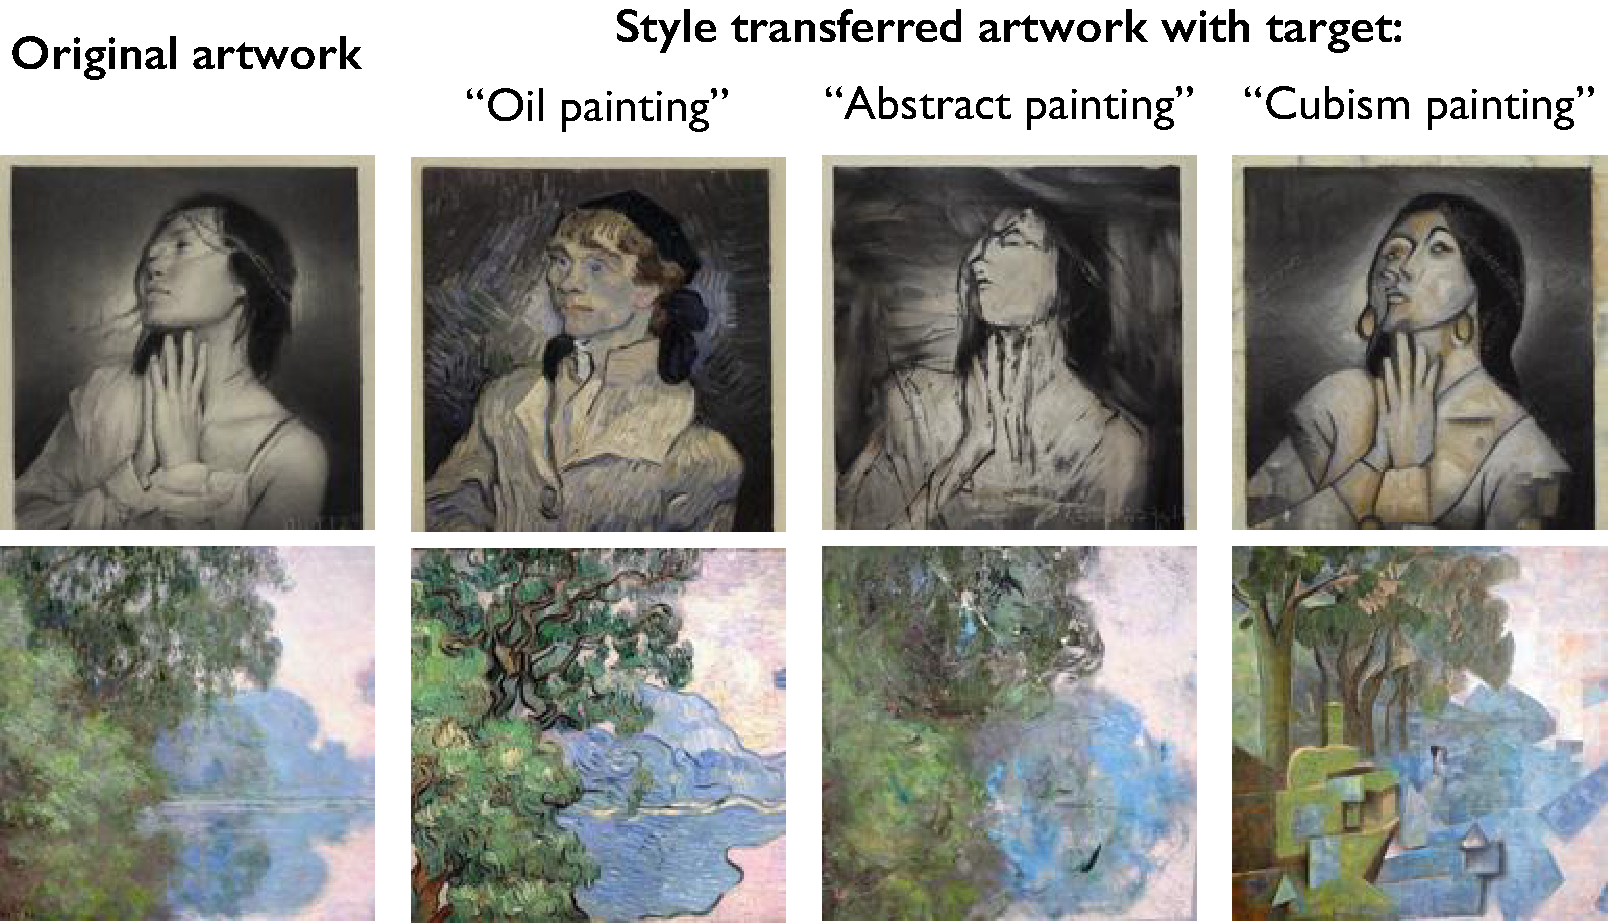
\includegraphics[width=1\columnwidth]{plots/eval/style-transfer-example.pdf}
  \caption{Example style-transferred artwork with different target styles. }
  \label{fig:transfer-examples}
\end{figure}

\secspace
\section{Disrupting Style Mimicry with Glaze} 
\label{sec:design}

In this section, we introduce \system{}, its design intuition followed by the
detailed algorithm. 

\secspace
\subsection{Design Intuition}
\label{sec:intuition-cloak}

Our key intuition is to identify and isolate \textit{style-specific features}
of an artist's original artwork, \ie the set of image features that
correspond to artistic style. Then \system{} computes cloaks while focusing
the perturbation budget on these style-specific features to maximize impact
on stylistic features.

As discussed, identifying and calculating style-specific features in model's
feature space is difficult due to the poor interpretability of model features
and how art style manifests differently across artworks. We overcome these two
challenges by designing a style-dependent and artwork-dependent method that
operates at image space. Given an artwork, we leverage ``style transfer,'' an
end-to-end computer vision technique, to modify and isolate its style
components. ``Style transfer'' transforms an image into a new image with a
different style (\eg from impressionist style to cubist style) while keeping
other aspects of the image similar (\eg subject matter and location).
% This is ideal for our use case, where protection must focus
% on style-specific features.

We leverage style transfer in our protection technique as follows. Given an
original artwork from the victim artist, we apply style-transfer to produce a
similar piece of art with a different style, \eg in style of ``an oil
painting by Van Gogh'' (Figure~\ref{fig:cloak-intuition} a). The new
version has similar content to the original, but its style mirrors that
of Van Gogh. We show more style-transfer examples with different target styles in
Figure~\ref{fig:transfer-examples}. Now, we can use the style-transferred
artwork as projection target to guide the perturbation computation. This
perturbs the original artwork's style-specific features towards that of
the style-transferred version. We do this by optimizing a cloak that, when
added to the original artwork, makes its feature representation similar to
the style-transferred image. Since the content is identical between the pair
of images, cloak optimization will focus its perturbation budget on style
features. 

\secspace
\subsection{Computing Style Cloaks} 

Using this approach, we compute style cloaks to disrupt style mimicry as
follows. Given an artwork ($x$), we use an existing feature extractor to
compute the style-transferred version of $x$ into target style $T$: $\Omega(x, T)$.
%style-transfer neural network that style transfers image $x$ and outputs
We then compute a style cloak $\delta_x$, such that $\delta_x$ moves $x$'s
style-specific feature representation to match that of $\Omega(x, T)$ while
minimizing visual impact. The cloak generation optimization is:

\secspace
\begin{eqnarray}
   &\min\limits_{\delta_x} Dist\left( \Phi(x + \delta_x), \Phi (\Omega(x, T))\right),  \label{eq:cloakopt}\\
  & \text{subject to } \; |\delta_x|< p, \nonumber
\end{eqnarray} 

\noindent where $\Phi$ is a generic image feature extractor commonly used in
text-to-image generation tasks, $Dist(.)$ computes the distance of two
feature representations, $|\delta_x|$ measures the perceptual perturbation
caused by cloaking, and $p$ is the perceptual perturbation budget. 

As discussed in \S\ref{sec:intuition-cloak}, the use of the style-transferred
image $\Omega(x, T)$ guides the cloak optimization in Eq~(\ref{eq:cloakopt})
to focus on changing style-specific image features. To maximize cloak
efficacy, the target style $T$ should be dissimilar from artist's original
style in the feature space. We discuss our heuristic for selecting target styles in
\S\ref{sec:design}.

\secspace
\subsection{Detailed System Design}
\label{sec:design-details}

Now we present the detailed design of \system{}. Given a victim
artist $V$, \system{} takes as input the set of $V$'s artwork to be shared
online $X_V$, an image feature extractor $\Phi$, a style-transfer model
$\Omega$, and perturbation budget $p$. Note that in many cases, a single
model (e.g. Stable Diffusion) provides both $\Phi$ and $\Omega$.

\para{Step 1: Choose Target Style.}  The selected target style $T$
should be sufficiently different from $V$'s style in model feature space to
maximize chances of disrupting style mimicry. For example, Fauvism and
Impressionism are distinct art styles that often look visually similar to the
untrained eye. Image of an impressionist painting style cloaked to Fauvism
might not produce a visually discernible effect on model-generated
paintings. Note that an artist can maximize their ability to avoid mimicry if
they consistently style cloak all their artwork towards the same target $T$.

For a new user, \system{} uses the following algorithm to randomly select $T$ from a set
of candidate styles reasonably different from $V$'s style. The algorithm
first inspects a public dataset of artists, each with a specific style (\eg
Monet, Van Gogh, Picasso). For each candidate target artist/style, it selects
a few images in that style and calculates their feature space centroid using
$\Phi$. It also computes $V$'s centroid in $\Phi$ using $V$'s artwork. Then,
it locates the set of candidate styles whose centroid distance to $V$'s
centroid is between the $50$ to $75$ percentile of all candidates. Finally,
it randomly selects $T$ from the candidate set.

\para{Step 2: Style transfer. } \system{} then leverages a pre-trained
style-transfer model $\Omega$~\cite{rombach2022high} to generate the
style-transferred artwork for optimization. Given each art piece $x \in
X_V$ and target style $T$, it style transfers $x$ to target style $T$ to
produce style-transferred image $\Omega(x, T)$.  

\para{Step 3: Compute cloak perturbation.} Then, \system{} computes the
cloak perturbation, $\delta_x$ for $x$, following the optimization defined
by eq. (\ref{eq:cloakopt}), subject to $|\delta_x| < p$. Our implementation
uses LPIPS (Learned Perceptual Image Patch
Similarity)~\cite{zhang2018unreasonable} to bound the perturbation. Different
from the $L_p$ distance used in previous
work~\cite{carlini2017towards,kurakin2016adversarial,sabour2015adversarial},
LPIPS has gained popularity as a measure of user-perceived image
distortion~\cite{cherepanova2021lowkey,laidlaw2020perceptual,rony2021augmented}. Bounding
cloak generation with this metric ensures that cloaked versions of images are
visually similar to the originals. We apply the \textit{penalty
  method}~\cite{nocedal2006numerical} to solve the optimization in
eq.(\ref{eq:cloakopt}) as follows:  

\vspace{-0.05in}
\begin{equation} \label{eq:optdetail} \vspace{-0.03in} 
 \underset{\delta_x}{\text{min }}||\Phi(\Omega(x, T)), \Phi(x + \delta_x) ||_2^2 + \alpha \cdot max(LPIPS(\delta_x)-p, 0) 
\end{equation}

\noindent where $\alpha$ controls the impact of the input perturbation. $L_2$
distance is used to calculate feature space distance.

\para{Upload artwork online.} Finally, the artist posts the cloaked artwork
online. For artists already with a large online presence, they can cloak and
re-upload artwork on their online portfolio.
While updating online images is not always possible, 
\system{} can be effective even when the mimic's model has significant amount
of uncloaked art (\S\ref{sec:robust-eval}).

\secspace
\subsection{On the Efficacy of Style Cloaks}
\label{sec:cloak-effect}

\system's style cloaks work by shifting feature representation of artwork in
the generator model. But how much shift do we need in order to have a
noticeable impact on mimicked art?


Two reasons suggest that even small shifts in style will have a meaningful
impact in disrupting style mimicry. First, generative models used for style
mimicry have {\em continuous} output spaces, \ie any shift in image feature
representation results in changes in the generated image.  Because generative
models are trained to interpolate their continuous feature
spaces~\cite{white2016sampling,upchurch2017deep}, any shift in the model's
representation of art style results in a new style, a ``blend'' between the
artist and the chosen target style.  
% the cloaked image with an \textbf{in-between style}, \ie a blended style of
% the original and target style,
Second, mimicked artwork must achieve reasonable quality and similarity in
style to the artist to be useful. Small shifts in the style space often
produce incoherent blends of conflicting styles that are enough to disrupt
style mimicry, \eg thick oil brushstrokes of Van Gogh's style mixed into a realism portrait.

These two factors contribute to \system{}'s success in more challenging
scenarios (\S\ref{sec:robust-eval}), and its robustness against
countermeasures (e.g. adversarial training) that succeed against cloaking
tools for facial recognition (\S\ref{sec:counter}).

